\documentclass{article}
\usepackage[papersize={216mm,330mm},left=0.8cm,top=0.5cm,right=0.8cm,bottom=1.2cm]{geometry}

\usepackage{amsmath}
\usepackage{amssymb}
\usepackage[american]{circuitikz}
\usepackage{enumerate}
\usepackage{tikz}
\usepackage{siunitx}
\usepackage{booktabs}
\usepackage{tcolorbox}
\usepackage{fancyhdr}
\usetikzlibrary{arrows.meta, calc}
\usepackage{enumitem}

\geometry{
  hmargin = {0.5cm, 0.6cm},
  vmargin = {1cm, -1cm},
  headsep = 2mm,
  head = 0cm,
  includeall,
  nomarginpar,
  foot = 1.5cm
}

\newcommand{\eps}{\varepsilon_0}
\newcommand{\ke}{k_e}

\tikzset{
  ejeflecha/.style   = {->, black, thick},
  guia/.style        = {black, dashed, thin},
  dim/.style         = {<->, black, thin}
}

\begin{document}

% ============================================================================
% PROPUESTA  - VERSION 1 - ENUNCIADO
% ============================================================================
\begin{enumerate}
 \item[3.] \textcolor{red}{(\textbf{20 pts})} En el plano $xy$ se tiene un cuarto de anillo de radio $R=0{,}5\,\text{m}$,
 centrado en el origen $O$ y ubicado en el primer cuadrante,
 con densidad  de carga lineal uniforme $\lambda_1 = 6\,\text{nC/m}$.
 Sobre el eje $+y$, desde $y=R$ hasta $y=5R$, se encuentra una varilla cargada uniformemente,
 cuya carga total es $Q_2=-4\,\text{nC}$.
Ambas distribuciones de carga se muestra en la figura.\\
 Determine:

\begin{minipage}{0.52\textwidth}
\begin{enumerate}[label={\alph*)}]
  \item La carga total $Q_1$ del cuarto de anillo. \textcolor{red}{(\textbf{4 pts})}
  \item La densidad lineal de carga $\lambda_2$ de la varilla. \textcolor{red}{(\textbf{4 pts})}
  \item El campo eléctrico en el origen generado por el cuarto de anillo.
        \textcolor{red}{(\textbf{6 pts})}
  \item El campo eléctrico en el origen generado por la varilla. \textcolor{red}{(\textbf{6 pts})}
\end{enumerate}
\end{minipage}
\hfill
\begin{minipage}{0.46\textwidth}
\begin{center}
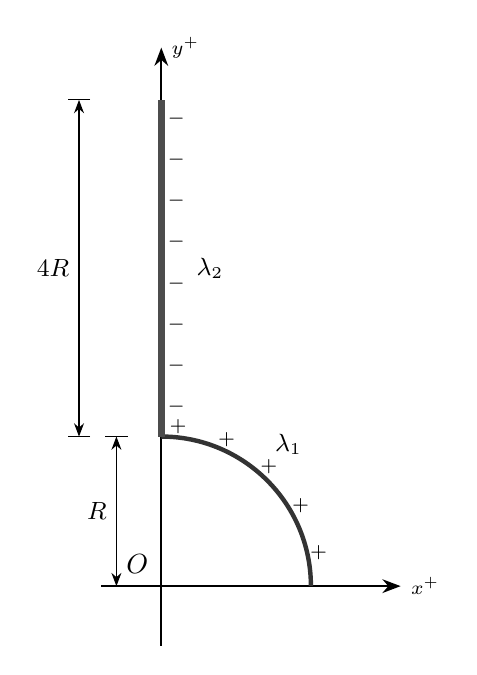
\begin{tikzpicture}[>=Stealth, thick, scale=0.95]
  \coordinate (O) at (0,0);

  \draw[ejeflecha] (-0.8,0) -- (3.2,0) node[right, font=\scriptsize]{$x^+$};
  \draw[ejeflecha] (0,-0.8) -- (0,7.2) node[right, font=\scriptsize]{$y^+$};

  \draw[line width=1.6pt, black!80] (2,0) arc[start angle=0, end angle=90, radius=2];
  \foreach \ang in {12,30,48,66,84}{
    \node[font=\scriptsize] at (\ang:2.15) {$+$};
  }
  \node[font=\small] at (1.7,1.9) {$\lambda_1$};

  \draw[line width=2.6pt, black!70] (0,2) -- (0,6.5);
  \foreach \y in {2.4,2.95,3.5,4.05,4.6,5.15,5.7,6.25}{
    \node[font=\scriptsize] at (0.2,\y) {$-$};
  }
  \node[font=\small] at (0.65,4.25) {$\lambda_2$};

  \node[font=\normalsize\bfseries, above left=1pt] at (O) {$O$};

  \draw[dim] (-0.6,0) -- (-0.6,2) node[midway, left, font=\small]{$R$};
  \draw[black, thin] (-0.45,0)--(-0.75,0);
  \draw[black, thin] (-0.45,2)--(-0.75,2);

  \draw[dim] (-1.1,2) -- (-1.1,6.5) node[midway, left, font=\small]{$4R$};
  \draw[black, thin] (-0.95,2)--(-1.25,2);
  \draw[black, thin] (-0.95,6.5)--(-1.25,6.5);
\end{tikzpicture}
\end{center}
\end{minipage}
\end{enumerate}

\newpage
\begin{center}
\textbf{Pauta versión 1}
\end{center}

\begin{enumerate}[label={\alph*)}]

\item \textbf{La carga total $Q_1$ del cuarto de anillo.
      \textcolor{red}{(\textbf{4 pts})}}

Parametrizando el cuarto de anillo mediante $0\leq\theta\leq\pi/2$, se tiene
$dl'=R\,d\theta$ y, por tanto, $dq=\lambda_1R\,d\theta$. Así,
\begin{eqnarray*}
  Q_1 &=& \int dq=\int_0^{\pi/2}\lambda_1R\,d\theta
  \quad{\color{red}(\textbf{1 pt})}
  \\[4pt]
  &=& \lambda_1R\left[\theta\right]_0^{\pi/2}
  =\frac{\lambda_1\pi R}{2}
  \quad{\color{red}(\textbf{1 pt})}\\[4pt]
  &=& \frac{(6\,\text{nC/m})\pi(0{,}5\,\text{m})}{2}
  =\boxed{1{,}5\pi\,\text{nC}\approx4{,}71\,\text{nC}}.
  \quad{\color{red}(\textbf{2 pts})}
\end{eqnarray*}

\item \textbf{La densidad lineal de carga $\lambda_2$ de la varilla.
      \textcolor{red}{(\textbf{4 pts})}}

Como la densidad es uniforme, $dq=\lambda_2\,dy'$. Integrando sobre la varilla,
\begin{eqnarray*}
  Q_2 &=& \int dq=\int_R^{5R}\lambda_2\,dy'
  \quad{\color{red}(\textbf{1 pt})}\\[4pt]
  Q_2 &=& \lambda_2\left[y'\right]_R^{5R}=4R\lambda_2
  \quad{\color{red}(\textbf{1 pt})}\\[4pt]
  \lambda_2 &=& \frac{Q_2}{4R}
  =\frac{-4\,\text{nC}}{4(0{,}5\,\text{m})}
  =\boxed{-2\,\text{nC/m}}.
  \quad{\color{red}(\textbf{2 pts})}
\end{eqnarray*}

% ─── a) ────────────────────────────────────────────────────────────────
\item \textbf{El campo eléctrico $\vec E_1(O)$ que genera el cuarto de anillo.
      \textcolor{red}{(\textbf{6 pts})}}

Usando la definición del campo eléctrico,
\begin{eqnarray*}
  d\vec{E}(\vec{r}) &=& \ke\frac{dq\left(\vec{r}-\vec{r}\,'\right)}{\|\vec{r}-\vec{r}\,'\|^3},
\end{eqnarray*}

\begin{itemize}[leftmargin=2em, itemsep=4pt]
  \item $\vec r = \vec 0$,\quad vector posición del punto de evaluación $O$.

  \item $\vec r\,' = R\cos\theta\,\hat\imath + R\sin\theta\,\hat\jmath$,\quad con
        $0\le\theta\le\pi/2$,\quad vector posición del elemento de carga sobre el arco.
        $\quad{\color{red}(\textbf{1 pt})}$

        Luego,
        \begin{eqnarray*}
          \vec r - \vec r\,' &=& -R\cos\theta\,\hat\imath - R\sin\theta\,\hat\jmath,
          \\[4pt]
          \|\vec r-\vec r\,'\| &=& R \quad\text{(constante, radio del arco)}.
          \quad{\color{red}(\textbf{1 pt})}
        \end{eqnarray*}

  \item $dq = \lambda_1\,dl' = \lambda_1 R\,d\theta$,\quad diferencial de carga.
        $\quad{\color{red}(\textbf{1 pt})}$
\end{itemize}

\medskip
Reemplazando e integrando sobre $\theta\in[0,\pi/2]$:
\begin{eqnarray*}
  \vec E_1(O) &=& \ke\int_0^{\pi/2}
      \frac{\lambda_1 R\,d\theta\,(-R\cos\theta\,\hat\imath-R\sin\theta\,\hat\jmath)}{R^3},\\[6pt]
  &=& \frac{\ke\lambda_1}{R}\left[-\big[\sin\theta\big]_0^{\pi/2}\hat\imath
      +\big[\cos\theta\big]_0^{\pi/2}\hat\jmath\right]
   =  \frac{\ke\lambda_1}{R}\big[(-1)\hat\imath+(-1)\hat\jmath\big],\\[6pt]
  \vec E_1(O) &=& \boxed{-\frac{\ke\lambda_1}{R}\left(\hat\imath+\hat\jmath\right)}
  \quad{\color{red}(\textbf{2 pts})}
\end{eqnarray*}

Evaluando con $\ke=9\times10^9\,\text{N m}^2/\text{C}^2$, $\lambda_1=6\times10^{-9}\,\text{C/m}$,
$R=0{,}5\,\text{m}$:
\begin{eqnarray*}
  \frac{\ke\lambda_1}{R} = \frac{(9\times10^9)(6\times10^{-9})}{0{,}5}=108\,\text{N/C}
  \quad\Longrightarrow\quad
  \vec E_1(O) \approx \left(-108\,\hat\imath-108\,\hat\jmath\right)\,\text{N/C}.
  \quad{\color{red}(\textbf{1 pt})}
\end{eqnarray*}

% ─── b) ────────────────────────────────────────────────────────────────
\item \textbf{El campo eléctrico $\vec E_2(O)$ que genera la varilla.
      \textcolor{red}{(\textbf{6 pts})}}

\begin{itemize}[leftmargin=2em, itemsep=4pt]
  \item $\vec r\,' = y'\,\hat\jmath$,\quad con $R\le y'\le 5R$,\quad vector posición del elemento de
        carga sobre la varilla. $\quad{\color{red}(\textbf{1 pt})}$

        \begin{eqnarray*}
          \vec r-\vec r\,' &=& -y'\,\hat\jmath, \quad{\color{red}(\textbf{1 pt})}\\[4pt]
          \|\vec r-\vec r\,'\| &=& y'.
        \end{eqnarray*}

  \item $dq=\lambda_2\,dy'$,\quad diferencial de carga.
        $\quad{\color{red}(\textbf{1 pt})}$
\end{itemize}

\begin{eqnarray*}
  \vec E_2(O) &=& \ke\int_R^{5R}\frac{\lambda_2\,dy'(-y'\,\hat\jmath)}{y'^3}
      = -\ke\lambda_2\,\hat\jmath\left[-\frac1{y'}\right]_R^{5R}
      = -\ke\lambda_2\,\hat\jmath\left(-\frac1{5R}+\frac1R\right),\\[6pt]
  \vec E_2(O) &=& \boxed{-\frac{4\ke\lambda_2}{5R}\,\hat\jmath}
  \quad{\color{red}(\textbf{2 pts})}
\end{eqnarray*}

Evaluando con $\lambda_2=-2\times10^{-9}\,\text{C/m}$, obtenida en el ítem b):
\begin{eqnarray*}
  \vec E_2(O) &=& -\frac{4(9\times10^9)(-2\times10^{-9})}{5(0{,}5)}\,\hat\jmath
  \;\approx\; 28{,}8\,\hat\jmath\ \text{N/C}. \quad{\color{red}(\textbf{1 pt})}
\end{eqnarray*}
El signo positivo indica que esta contribución apunta en el sentido $+y$, hacia la varilla de carga negativa.

\end{enumerate}

% ============================================================================
% PROPUESTA - VERSION 2 - ENUNCIADO
% ============================================================================
\newpage
\begin{enumerate} 
 \item[3.] \textcolor{red}{(\textbf{20 pts})} En el plano $xy$ se tiene un cuarto de anillo de
 radio $R=0{,}6\,\text{m}$, centrado en el origen $O$ y ubicado en el primer cuadrante, con densidad de carga lineal uniforme
 $\lambda_1 = -4\,\text{nC/m}$.
 Sobre el eje $+x$, desde $x=R$ hasta $x=4R$, se encuentra una varilla cargada uniformemente,
 cuya carga total es $Q_2=7{,}2\,\text{nC}$.
Ambas distribuciones de carga se muestra en la figura.\\
 Determine:

\begin{minipage}{0.52\textwidth}
\begin{enumerate}[label={\alph*)}]
  \item La carga total $Q_1$ del cuarto de anillo. \textcolor{red}{(\textbf{4 pts})}
  \item La densidad lineal de carga $\lambda_2$ de la varilla. \textcolor{red}{(\textbf{4 pts})}
  \item El campo eléctrico en el origen generado por el cuarto de anillo.
        \textcolor{red}{(\textbf{6 pts})}
  \item El campo eléctrico en el origen generado por la varilla. \textcolor{red}{(\textbf{6 pts})}
\end{enumerate}
\end{minipage}
\hfill
\begin{minipage}{0.46\textwidth}
\begin{center}
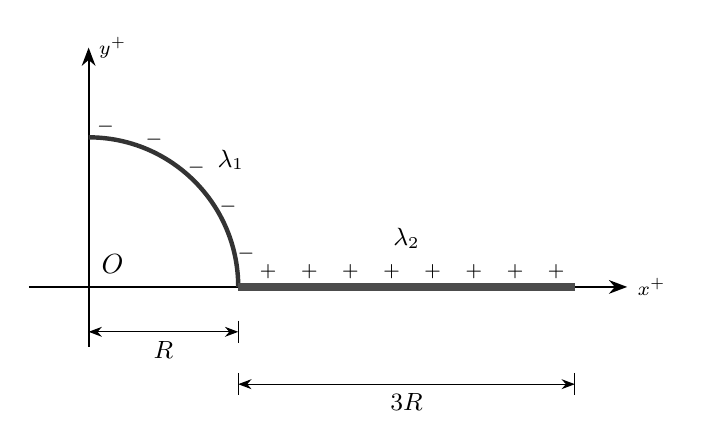
\begin{tikzpicture}[>=Stealth, thick, scale=0.95]
  \coordinate (O) at (0,0);

  \draw[ejeflecha] (-0.8,0) -- (7.2,0) node[right, font=\scriptsize]{$x^+$};
  \draw[ejeflecha] (0,-0.8) -- (0,3.2) node[right, font=\scriptsize]{$y^+$};

  \draw[line width=1.6pt, black!80] (2,0) arc[start angle=0, end angle=90, radius=2];
  \foreach \ang in {12,30,48,66,84}{
    \node[font=\scriptsize] at (\ang:2.15) {$-$};
  }
  \node[font=\small] at (1.9,1.7) {$\lambda_1$};

  \draw[line width=2.6pt, black!70] (2,0) -- (6.5,0);
  \foreach \x in {2.4,2.95,3.5,4.05,4.6,5.15,5.7,6.25}{
    \node[font=\scriptsize] at (\x,0.2) {$+$};
  }
  \node[font=\small] at (4.25,0.65) {$\lambda_2$};

  \node[font=\normalsize\bfseries, above right=1pt] at (O) {$O$};

  \draw[dim] (0,-0.6) -- (2,-0.6) node[midway, below, font=\small]{$R$};
  \draw[black, thin] (0,-0.45)--(0,-0.75);
  \draw[black, thin] (2,-0.45)--(2,-0.75);

  \draw[dim] (2,-1.3) -- (6.5,-1.3) node[midway, below, font=\small]{$3R$};
  \draw[black, thin] (2,-1.15)--(2,-1.45);
  \draw[black, thin] (6.5,-1.15)--(6.5,-1.45);
\end{tikzpicture}
\end{center}
\end{minipage}
\end{enumerate}

\newpage
\begin{center}
\textbf{Pauta versión 2}
\end{center}

\begin{enumerate}[label={\alph*)}]

\item \textbf{La carga total $Q_1$ del cuarto de anillo.
      \textcolor{red}{(\textbf{4 pts})}}

Parametrizando el cuarto de anillo mediante $0\leq\theta\leq\pi/2$, se tiene
$dl'=R\,d\theta$ y, por tanto, $dq=\lambda_1R\,d\theta$. Así,
\begin{eqnarray*}
  Q_1 &=& \int dq=\int_0^{\pi/2}\lambda_1R\,d\theta
  \quad{\color{red}(\textbf{1 pt})}
  \\[4pt]
  &=& \lambda_1R\left[\theta\right]_0^{\pi/2}
  =\frac{\lambda_1\pi R}{2}
  \quad{\color{red}(\textbf{1 pt})}\\[4pt]
  &=& \frac{(-4\,\text{nC/m})\pi(0{,}6\,\text{m})}{2}
  =\boxed{-1{,}2\pi\,\text{nC}\approx-3{,}77\,\text{nC}}.
  \quad{\color{red}(\textbf{2 pts})}
\end{eqnarray*}

\item \textbf{La densidad lineal de carga $\lambda_2$ de la varilla.
      \textcolor{red}{(\textbf{4 pts})}}

Como la densidad es uniforme, $dq=\lambda_2\,dx'$. Integrando sobre la varilla,
\begin{eqnarray*}
  Q_2 &=& \int dq=\int_R^{4R}\lambda_2\,dx'
  \quad{\color{red}(\textbf{1 pt})}\\[4pt]
  Q_2 &=& \lambda_2\left[x'\right]_R^{4R}=3R\lambda_2
  \quad{\color{red}(\textbf{1 pt})}\\[4pt]
  \lambda_2 &=& \frac{Q_2}{3R}
  =\frac{7{,}2\,\text{nC}}{3(0{,}6\,\text{m})}
  =\boxed{4\,\text{nC/m}}.
  \quad{\color{red}(\textbf{2 pts})}
\end{eqnarray*}

% ─── a) ────────────────────────────────────────────────────────────────
\item \textbf{El campo eléctrico $\vec E_1(O)$ que genera el cuarto de anillo.
      \textcolor{red}{(\textbf{6 pts})}}

Usando la definición del campo eléctrico,
\begin{eqnarray*}
  d\vec{E}(\vec{r}) &=& \ke\frac{dq\left(\vec{r}-\vec{r}\,'\right)}{\|\vec{r}-\vec{r}\,'\|^3},
\end{eqnarray*}

\begin{itemize}[leftmargin=2em, itemsep=4pt]
  \item $\vec r = \vec 0$,\quad vector posición del punto de evaluación $O$.

  \item $\vec r\,' = R\cos\theta\,\hat\imath + R\sin\theta\,\hat\jmath$,\quad con
        $0\le\theta\le\pi/2$,\quad vector posición del elemento de carga sobre el arco.
        $\quad{\color{red}(\textbf{1 pt})}$

        Luego,
        \begin{eqnarray*}
          \vec r - \vec r\,' &=& -R\cos\theta\,\hat\imath - R\sin\theta\,\hat\jmath,
          \\[4pt]
          \|\vec r-\vec r\,'\| &=& R \quad\text{(constante, radio del arco)}.
          \quad{\color{red}(\textbf{1 pt})}
        \end{eqnarray*}

  \item $dq = \lambda_1\,dl' = \lambda_1 R\,d\theta$,\quad diferencial de carga.
        $\quad{\color{red}(\textbf{1 pt})}$
\end{itemize}

\medskip
Reemplazando e integrando sobre $\theta\in[0,\pi/2]$:
\begin{eqnarray*}
  \vec E_1(O) &=& \ke\int_0^{\pi/2}\frac{\lambda_1 R\,d\theta\,(-R\cos\theta\,\hat\imath
      -R\sin\theta\,\hat\jmath)}{R^3},\\[6pt]
  &=& \frac{\ke\lambda_1}{R}\left[-\big[\sin\theta\big]_0^{\pi/2}\hat\imath
      +\big[\cos\theta\big]_0^{\pi/2}\hat\jmath\right]
   = \frac{\ke\lambda_1}{R}\big[(-1)\hat\imath+(-1)\hat\jmath\big],\\[6pt]
  \vec E_1(O) &=& \boxed{-\frac{\ke\lambda_1}{R}\left(\hat\imath+\hat\jmath\right)}
  \quad{\color{red}(\textbf{2 pts})}
\end{eqnarray*}

Evaluando con $\ke=9\times10^9\,\text{N m}^2/\text{C}^2$, $\lambda_1=-4\times10^{-9}\,\text{C/m}$,
$R=0{,}6\,\text{m}$:
\begin{eqnarray*}
  \frac{\ke\lambda_1}{R} &=& \frac{(9\times10^9)(-4\times10^{-9})}{0{,}6}=-60\,\text{N/C},\\[4pt]
  \vec E_1(O) &\approx& \left(60\,\hat\imath+60\,\hat\jmath\right)\,\text{N/C}.
  \quad{\color{red}(\textbf{1 pt})}
\end{eqnarray*}

% ─── b) ────────────────────────────────────────────────────────────────
\item \textbf{El campo eléctrico $\vec E_2(O)$ que genera la varilla.
      \textcolor{red}{(\textbf{6 pts})}}

\begin{itemize}[leftmargin=2em, itemsep=4pt]
  \item $\vec r\,' = x'\,\hat\imath$,\quad con $R\le x'\le 4R$,\quad vector posición del elemento de
        carga sobre la varilla. $\quad{\color{red}(\textbf{1 pt})}$

        \begin{eqnarray*}
          \vec r-\vec r\,' &=& -x'\,\hat\imath, \quad{\color{red}(\textbf{1 pt})}\\[4pt]
          \|\vec r-\vec r\,'\| &=& x'.
        \end{eqnarray*}

  \item $dq=\lambda_2\,dx'$,\quad diferencial de carga.
        $\quad{\color{red}(\textbf{1 pt})}$
\end{itemize}

\begin{eqnarray*}
  \vec E_2(O) &=& \ke\int_R^{4R}\frac{\lambda_2\,dx'(-x'\,\hat\imath)}{x'^3}
      = -\ke\lambda_2\,\hat\imath\left[-\frac1{x'}\right]_R^{4R}
      = -\ke\lambda_2\,\hat\imath\left(-\frac1{4R}+\frac1R\right),\\[6pt]
  \vec E_2(O) &=& \boxed{-\frac{3\ke\lambda_2}{4R}\,\hat\imath}
  \quad{\color{red}(\textbf{2 pts})}
\end{eqnarray*}

Evaluando con $\lambda_2=4\times10^{-9}\,\text{C/m}$, obtenida en el ítem b):
\begin{eqnarray*}
  \vec E_2(O) &=& -\frac{3(9\times10^9)(4\times10^{-9})}{4(0{,}6)}\,\hat\imath
  \;\approx\; -45\,\hat\imath\ \text{N/C}. \quad{\color{red}(\textbf{1 pt})}
\end{eqnarray*}
El signo negativo indica que esta contribución apunta en el sentido $-x$, alejándose de la varilla de carga positiva.

\end{enumerate}

\end{document}
